\documentclass[tikz]{standalone}

\usepackage{tikz}
\usetikzlibrary{calc}
\usetikzlibrary{arrows.meta}

\begin{document}
    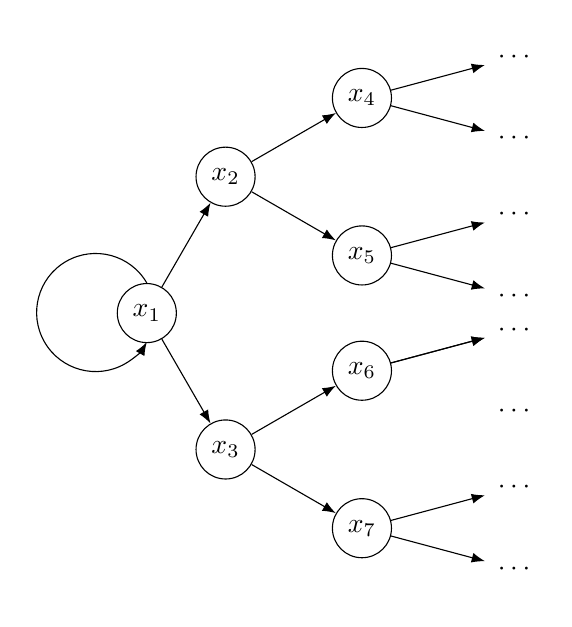
\begin{tikzpicture}
        [
        remember picture,
        every node/.style={draw,circle,minimum size=0.75cm,inner sep=-1pt},
        >=Latex
        ]
        \node (x1) at (0,0) {$x_1$};
        \node (x2) at ($(x1) + (60:2)$) {$x_2$};
        \node (x3) at ($(x1) + (-60:2)$) {$x_3$};
        \node (x4) at ($(x2) + (30:2)$) {$x_4$};
        \node (x5) at ($(x2) + (-30:2)$) {$x_5$};
        \node (x6) at ($(x3) + (30:2)$) {$x_6$};
        \node (x7) at ($(x3) + (-30:2)$) {$x_7$};

        \node[draw=none] (x8)  at ($(x4) + (15:2)$)  {$\cdots$};
        \node[draw=none] (x9)  at ($(x4) + (-15:2)$) {$\cdots$};
        \node[draw=none] (x10) at ($(x5) + (15:2)$)  {$\cdots$};
        \node[draw=none] (x11) at ($(x5) + (-15:2)$) {$\cdots$};
        \node[draw=none] (x12) at ($(x6) + (15:2)$)  {$\cdots$};
        \node[draw=none] (x13) at ($(x6) + (-15:2)$) {$\cdots$};
        \node[draw=none] (x14) at ($(x7) + (15:2)$)  {$\cdots$};
        \node[draw=none] (x15) at ($(x7) + (-15:2)$) {$\cdots$};


        \draw[->] (x1) -- (x2);
        \draw[->] (x1) -- (x3);
        \draw[->] (x2) -- (x4);
        \draw[->] (x2) -- (x5);
        \draw[->] (x3) -- (x6);
        \draw[->] (x3) -- (x7);
        \draw[->] (x4) -- (x8);
        \draw[->] (x4) -- (x9);
        \draw[->] (x5) -- (x10);
        \draw[->] (x5) -- (x11);
        \draw[->] (x6) -- (x12);
        \draw[->] (x6) -- (x12);
        \draw[->] (x7) -- (x14);
        \draw[->] (x7) -- (x15);
        \draw[->] (x1.north) arc(30:330:0.75);
    \end{tikzpicture}
\end{document}